\section{Data}

\subsection{Description}
The data used for clustering were drawn from the back office system of a travel agency in Parga, Greece. The majority of the data are about hotel reservations. The rest are about excursions and transfers. The back office uses a relational database to store its data. After thoroughly examining the available tables, only a few of them were kept for the analysis, the ones that seemed to have the most analytical value. Their relationships are shown in the following simplified diagram. \\
\begin{figure}[ht]
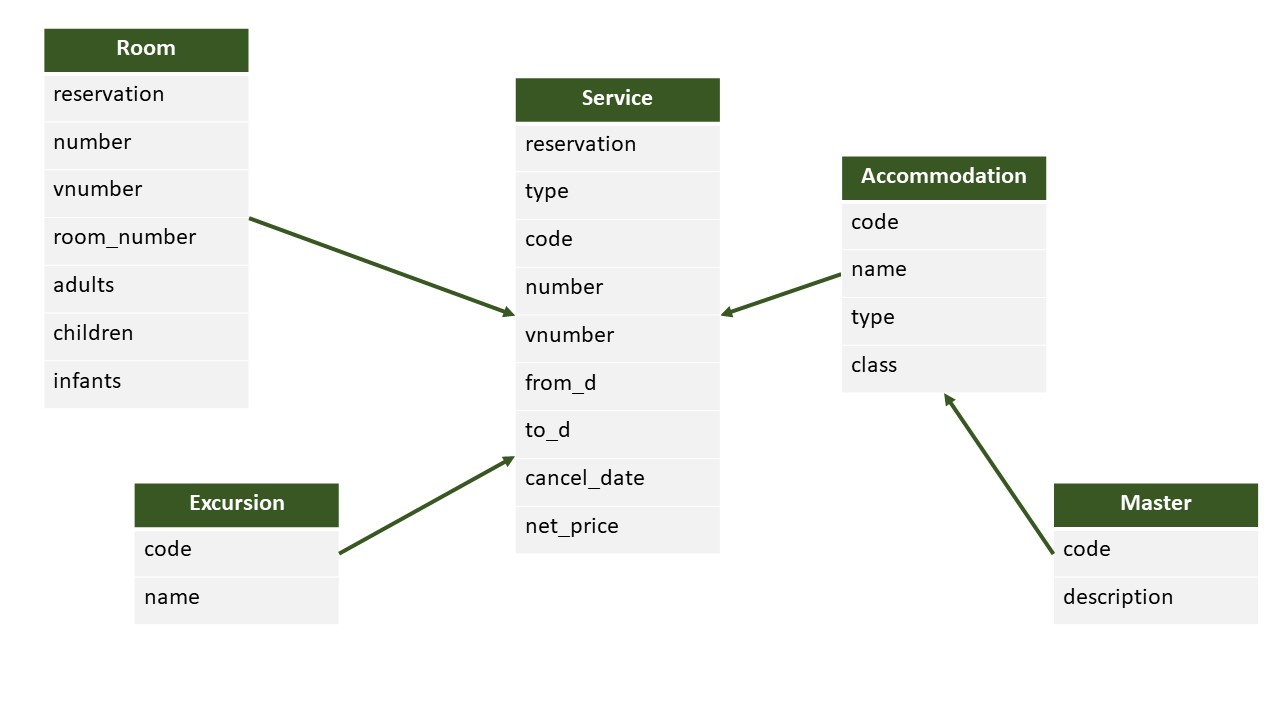
\includegraphics[width=\textwidth]{erp}
\caption{Relationships diagram.}
\label{fig:erp}
\end{figure}
\\
One reservation may consist of many services (e.g., hotel reservation, excursion activity). For each service booked, there is at least one corresponding row on the 'Service' table that contains its details in a total of sixty-seven columns. Eleven of them were used and are explained in table \ref{tab:service}. \\
\begin{table}[h!]
\begin{center}
\begin{tabular}{l | p{12cm}}
\textcolor{theme}{\textbf{Column}} & \textcolor{theme}{\textbf{Description}}\\
\hline
reservation & Service's reservation identifier.\\
\hline
type & Service type. Can be either hotel(HTL), excursion(EXC) or transfer(TRF).\\
\hline
code & Service code from either 'Excursion', 'Hotel', or 'Transfer' tables.\\
\hline
number & Service number. The service's identifier number per reservation.\\
\hline
vnumber & Service vnumber. A number starting from one for each service per reservation. Whenever the service is edited a new row is created with the updated details and vnumber incremented by one.\\
\hline
fromd & Service's starting date.\\
\hline
tod & Service's ending date.\\
\hline
net\_price & The total price of the booked service.\\
\hline
status & Reservation status. Can be either canceled(CL) or confirmed(CF). \\
\hline
customer\_id & Customer's identifier.\\
\hline
\end{tabular}
\caption{Service table.}
\label{tab:service}
\end{center}
\end{table}
\\
Whenever an accommodation service is booked, the "Accommodation"(\ref{tab:accommodation}) table, holds the information that describes it. Using the service code set on the "Service" table the corresponding accommodation can be found. \\
\begin{table}[h!]
\begin{center}
\begin{tabular}{l | p{12cm}}
\textcolor{theme}{\textbf{Column}} & \textcolor{theme}{\textbf{Description}}\\
\hline
code & Accommodation identifier.\\
\hline
name & Accommodation name.\\
\hline
type & Accommodation type identifier. Categorical value that shows the type of the accommodation. \\
\hline
class & Accommodation class identifier. Categorical value that shows the quality of the accommodation. \\
\hline
\end{tabular}
\caption{Accommodation table.}
\label{tab:accommodation}
\end{center}
\end{table}
\\
The "Master"(\ref{tab:master}) table contains several codes, and its descriptions, that can be found on many tables of the database, including the accommodation class and type codes. \\
\begin{table}[h!]
\begin{center}
\begin{tabular}{l | p{12cm}}
\textcolor{theme}{\textbf{Column}} & \textcolor{theme}{\textbf{Description}}\\
\hline
code & A code.\\
\hline
description & Code's description.\\
\hline
\end{tabular}
\caption{Master table.}
\label{tab:master}
\end{center}
\end{table}
\\
Furthermore, whenever an accommodation is booked, at least one new row is entered in 'Room' table. These rows contain the information of the booked rooms of the accommodation, as described in table \ref{tab:room}. \\
\begin{table}[h!]
\begin{center}
\begin{tabular}{l | p{12cm}}
\textcolor{theme}{\textbf{Column}} & \textcolor{theme}{\textbf{Description}}\\
\hline
reservation & Service's reservation identifier.\\
\hline
number & Service number. The service's identifier number per reservation.\\
\hline
vnumber & Service vnumber. A number starting from one for each service per reservation. Whenever the service is edited a new row is created with the updated details and vnumber incremented by one.\\
\hline
room\_number & The number of rooms contained in this service booking with this specific composition.\\
\hline
adults & The number of adults in this room.\\
\hline
children & The number of children in this room.\\
\hline
infants & The number of infants in this room.\\
\hline
\end{tabular}
\caption{Room table.}
\label{tab:room}
\end{center}
\end{table}
\\
Similarly to an accommodation booking, when an excurision is booked its details can be found through the service code of "Service" table in table \ref{tab:excursion}. \\
\begin{table}[h!]
\begin{center}
\begin{tabular}{l | p{12cm}}
\textcolor{theme}{\textbf{Column}} & \textcolor{theme}{\textbf{Description}}\\
\hline
code & Excursion identifier.\\
\hline
name & Excursion name.\\
\hline
\end{tabular}
\caption{Excursion table.}
\label{tab:excursion}
\end{center}
\end{table}
\\
\subsection{Processing and reforming}
After cleaning the data and before performing the analysis, some additional preprocessing was done. This preprocessing contained the creation of new columns and tranformation of categorical data to numerical, ordinal whenever that was possible.Eventually, the tables were reformed to a flat structure. The additional data were used both for the analysis and the interpretation of the results. \\
First of all, the service booking dates were used in order to define the season status of the trip. The season status can either be low, medium or high, and is used to show whether, in a certain period, a small or a big number of reservations is expected. As defined from the travel agency, high season is during Christmas and Easter(in this case orthodox) holidays and from the 10th of July to the end of August. Medium season are considered September, June and from the 1st until the 9th of July. The rest of the year is considered low season. Furthermore, in order to keep each booked service only once, on its final state, only the maximum vnumber was kept for each service. Finally, for the accommodation services, to get a more representative value of the service, the price per person per night was calculated. \\
As shown in figure \Nameref{fig:erp}, the 'Room' table contains information with regard to its composition. Instead of just using the number of adults and children a composition tag was created. The terms used by the travel agency to describe the composition are family, couple, single, crew and group. For interpration purposes these tags were added to the room data. \\
As already mentioned, information about the type and class can be drawn from the 'Master' table. The descriptions of the codes by themeselves provide many verbal information that can be summarized to create universal tags for the accommodations. Therefore, using those descriptions, five type tags were created, hotel, studio, apartment, house and villa, and three class tags, A(high class), B(medium class) or C(low class). The class tags were represented by numerical values for the analysis.
After transforming the initial tables to a flat structure, several plots were made with different combinations of columns and data formats using PCA(Principal Component Analysis). These plots helped to get a better idea of how the data are scattered and also test whether the data manipulation already done could result in meaningful clusters. The plot of the data that were later used for the analysis is shown in figure \ref{fig:PCA}. By observing the figure, we would expect as an ideal output of the algorithms four clusters. \\
\begin{figure}[ht]
\centering
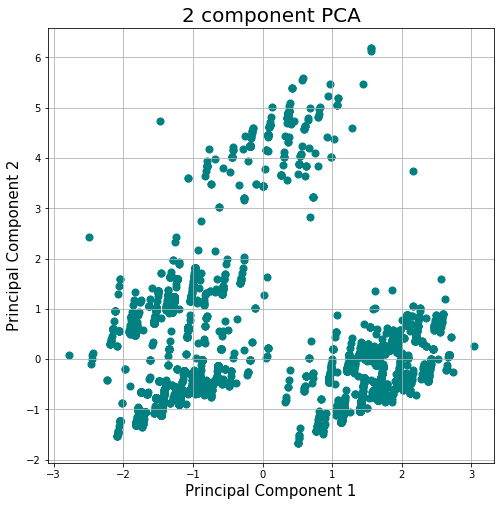
\includegraphics[width=9cm,height=9cm]{initial}
\caption{Data plot.}
\label{fig:PCA}
\end{figure}

\section{Kmeans}
The first algorithm used was Kmeans. The metric used to calculate the distances was Euclidean distance and the number of repetitions was 50. \\
Before running the algorithm, two methods were used to find the best number of clusters to be used for the value of k. The first one, the elbow method, returned that the ideal number of clusters is seven (\ref{fig:elbow}). The second one used was the silhouette method. In this case, the ideal number of k was eight as shown in diagram \ref{fig:shilouette}.
\begin{figure}[ht]
\centering
\begin{subfigure}{.5\textwidth}
\centering
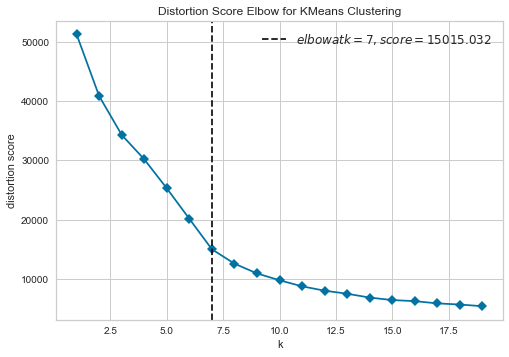
\includegraphics[width=\linewidth]{kmeans_elbow}
\caption{Elbow method.}
\label{fig:elbow}
\end{subfigure}%
\begin{subfigure}{.5\textwidth}
\centering
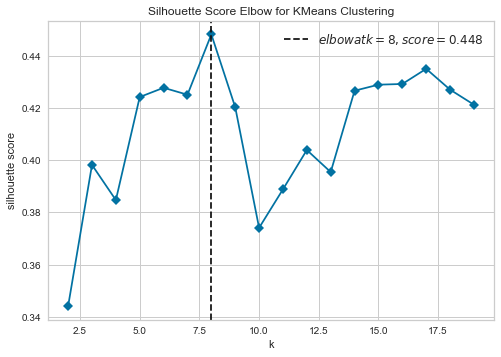
\includegraphics[width=\linewidth]{kmeans_shilouette}
\caption{Shilouette method.}
\label{fig:shilouette}
\end{subfigure}%
\caption{Methods used to find the optimal number of clusters.}
\label{fig:methods}
\end{figure}
\\
In order to conclude which would be the final kmeans clusters to be analyzed, kmeans was run two times, using as k the numbers seven and eight respectively. Afterward, PCA was used on both results and seven was chosen as the best fit. From the seven produced clusters three of them were considered unworthy of further analysis because they were too small. So eventually, kmeans resulted in four clusters that can be observed in figure \ref{fig:kmeans}. \\
\begin{figure}[ht]
\centering
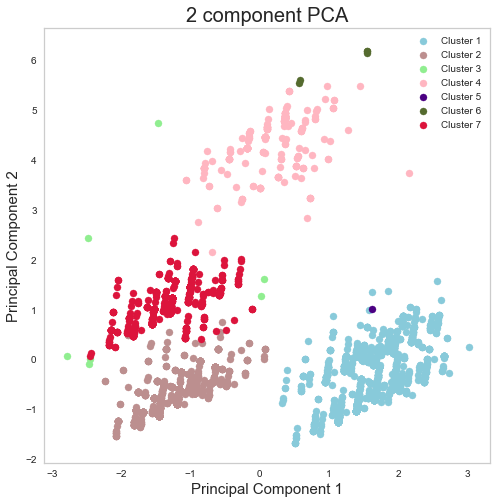
\includegraphics[width=9cm,height=9cm]{kmeans}
\caption{Kmeans algorithm.}
\label{fig:kmeans}
\end{figure}
\\
Descriptive statistics were used to better understand the created groups and the reasons why they were formed the way they did. The formation of the clusters was affected to a great extent by the type of accommodation. The type of accommodation was the only categorical data used for the analysis that could not be converted to ordinal, therefore it is normal that the algorithm recognized those groups. In the following paragraphs, the clusters will be analyzed. \\
The first cluster(cluster 1 in diagrams) mainly contains low-cost, brief trips done by either families, crews or groups. These trips are more 'Value for money' oriented, since, even though they are very cheap, they contain relatively good quality accommodations (category B). \\
The second one(cluster 2 in diagrams) is also for brief trips. It differentiates on the category of the accommodation, the cost, and the composition. It contains accommodations of the highest quality, of the highest cost of all the clusters, and includes mainly singles and couples. This is considered a cluster that describes 'Luxury trips'. \\
The third cluster(cluster 4 in diagrams) differentiates mainly from the others on the trip's number of days, which appears to be very high. The reservations are mainly for studios of average quality and price. This is the 'Relaxing vacation' cluster. \\
Finally, the last cluster(cluster 7 in diagrams) is very similar to the first one, apart from one very important factor. The quality of the accommodation is the lowest of all the other clusters even though the price does not change that much, as it can be observed from diagram \ref{fig:kmeans1}. This is the 'Cheap trip' cluster.
\begin{figure}[ht]
\centering
\begin{subfigure}{.5\textwidth}
\centering
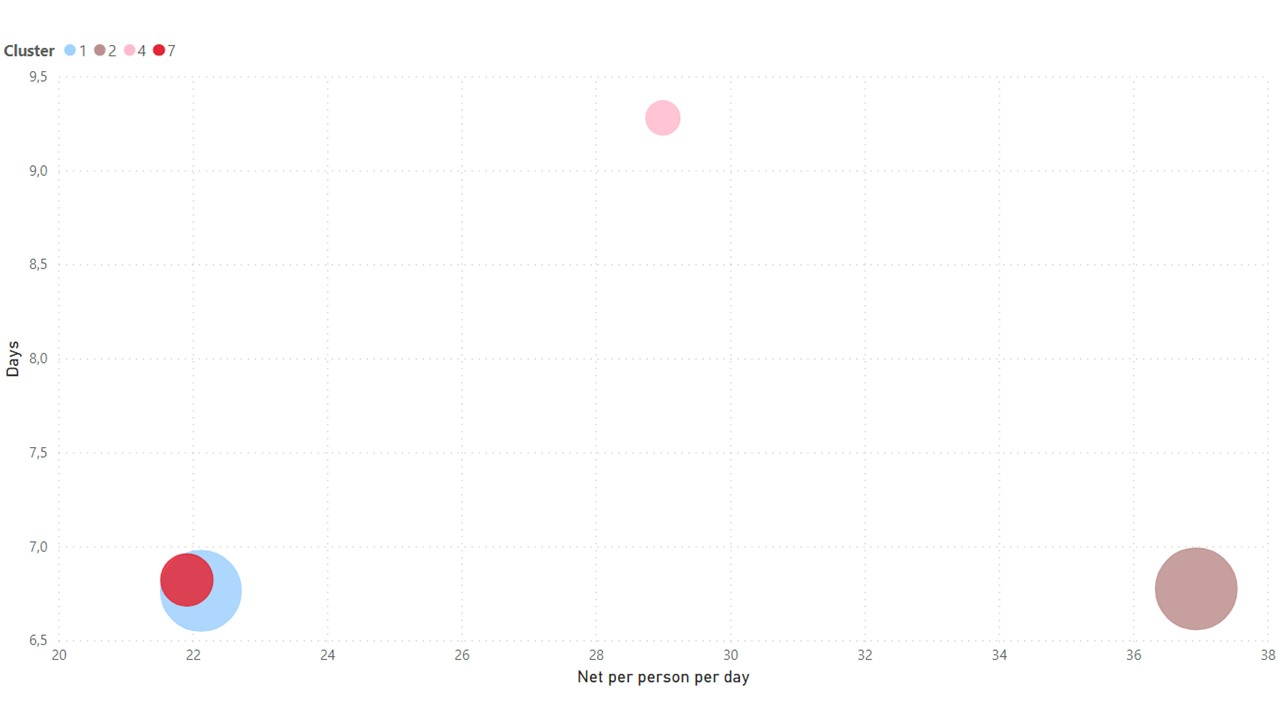
\includegraphics[width=\linewidth]{kmeans_diagram_1}
\caption{Average days and average net per person per day for each cluster.}
\label{fig:kmeans1}
\end{subfigure}%
\begin{subfigure}{.5\textwidth}
\centering
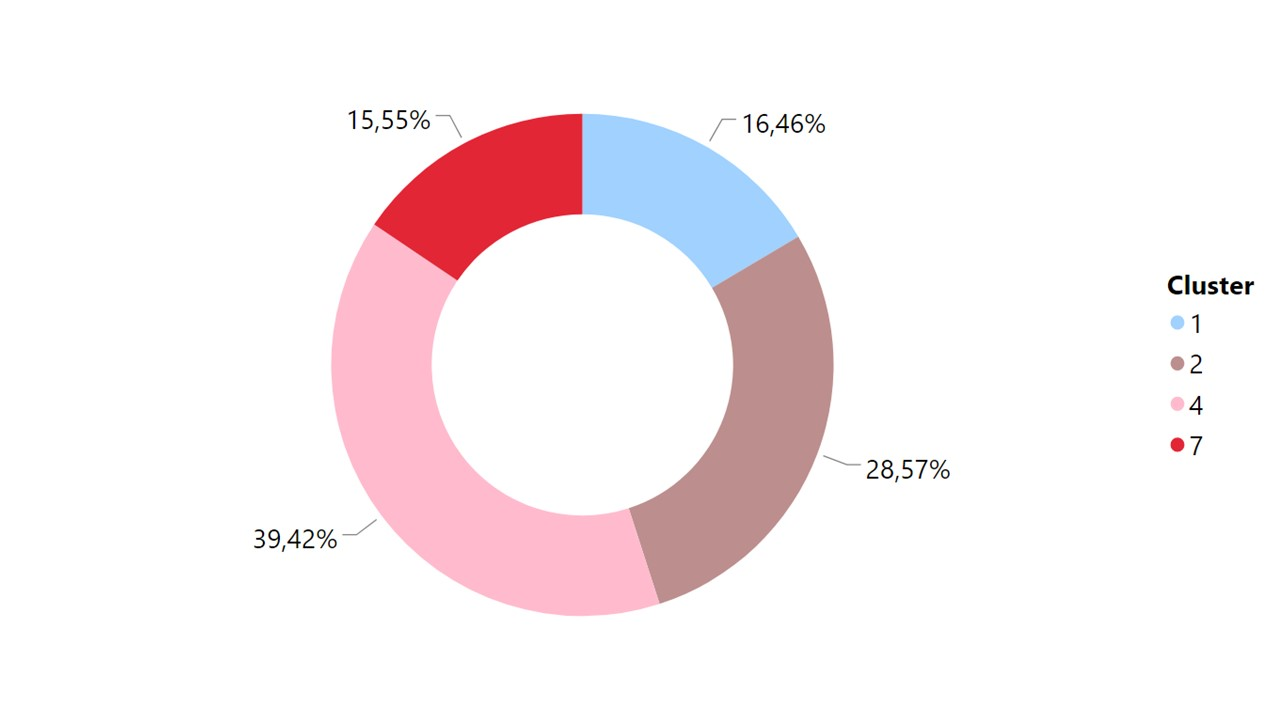
\includegraphics[width=\linewidth]{kmeans_diagram_2}
\caption{Total net for each cluster.}
\label{fig:kmeans2}
\end{subfigure}%
\caption{Descriptive statistics of the clusters.}
\label{fig:kmeans_descriptives}
\end{figure}
\\
As observed from diagram \ref{fig:kmeans2}, the most profitable for the agency clusters seem to be clusters 'Luxury trips' and 'Relaxing vacation'. Based on those results the agency could adjust the provided product more to the customer needs. Therefore, in order to increase profits, the travel agency could include more trips of these types to their portfolios. These results can also help in the way the agency addresses its clients. It could change its marketing campaigns to target each group in a more personalized way and attract more clients. For example, when targeting a family it could present its package as a smart value for money option. Furthermore, it could concentrate more on promoting the two most profitable groups, especially cluster number 4, which seems to be one of the most profitable while counting a small number of reservations. In this way, it could effectively increase its revenue. \\

\section{Agglomerative Clustering}
The second method used to cluster the dataset was Agglomerative clustering. The metric used to compute the linkage between the clusters was the Manhattan distance, using average linkage. To observe the formation of clusters the dendogram \ref{fig:dendrogram} was created. \\
\begin{figure}[ht]
\centering
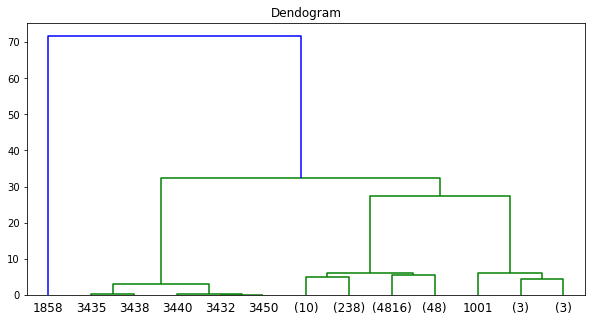
\includegraphics[width=0.7\linewidth,height=0.4\linewidth]{dendrogram}
\caption{Dendrogram.}
\label{fig:dendrogram}
\end{figure}
\\
 By observing it the expected clusters would be three. Though, PCA was also used for various values of n and eventually the number of clusters was set to eight, with the result being the following. \\
\begin{figure}[ht]
\centering
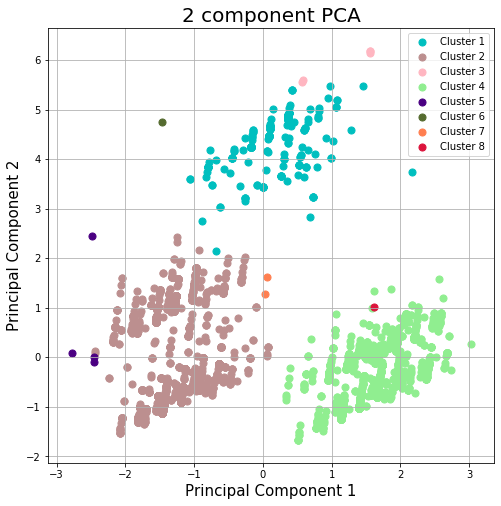
\includegraphics[width=9cm,height=9cm]{agglomerative}
\caption{Agglomerative clustering.}
\label{fig:agglomerative}
\end{figure}
\\
Just as in the case of Kmeans, some of the clusters formed did not provide meaningful results and were not considered worth analyzing. The ones that provide useful information are clusters one, two and four. Cluster 1 of agglomerative clustering is the 'Value for money' cluster from Kmeans, and cluster 4 is the 'Relaxing Vacation' cluster. Cluster 2 seems to be a join of the other two Kmeans clusters and will be named 'Low cost trip' cluster, since it contains the cheapest accommodations, of the lowest quality, and it is about trips that do not last many days (\ref{agglomerative_diagram_2}). 
\begin{figure}[ht]
\centering
\begin{subfigure}{.5\textwidth}
\centering
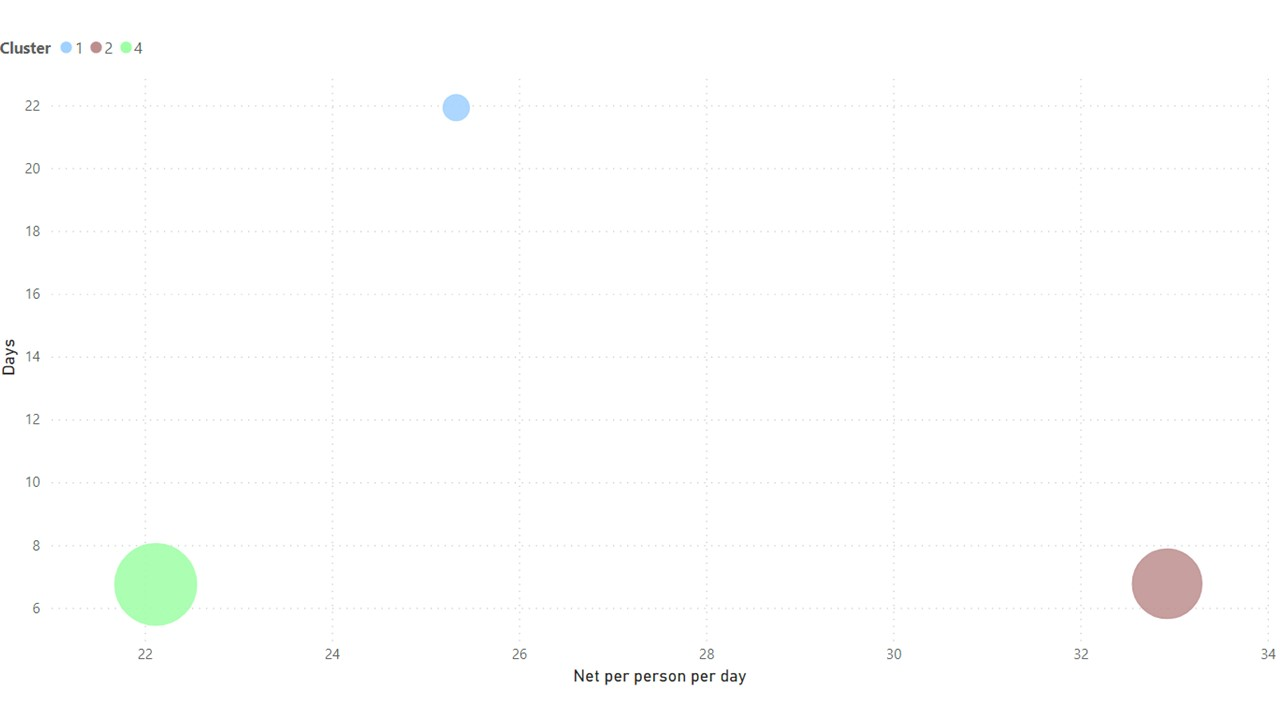
\includegraphics[width=\linewidth]{agglomerative_diagram_2}
\caption{Average days and average net per person per day for each cluster.}
\label{fig:agglomerative1}
\end{subfigure}%
\begin{subfigure}{.5\textwidth}
\centering
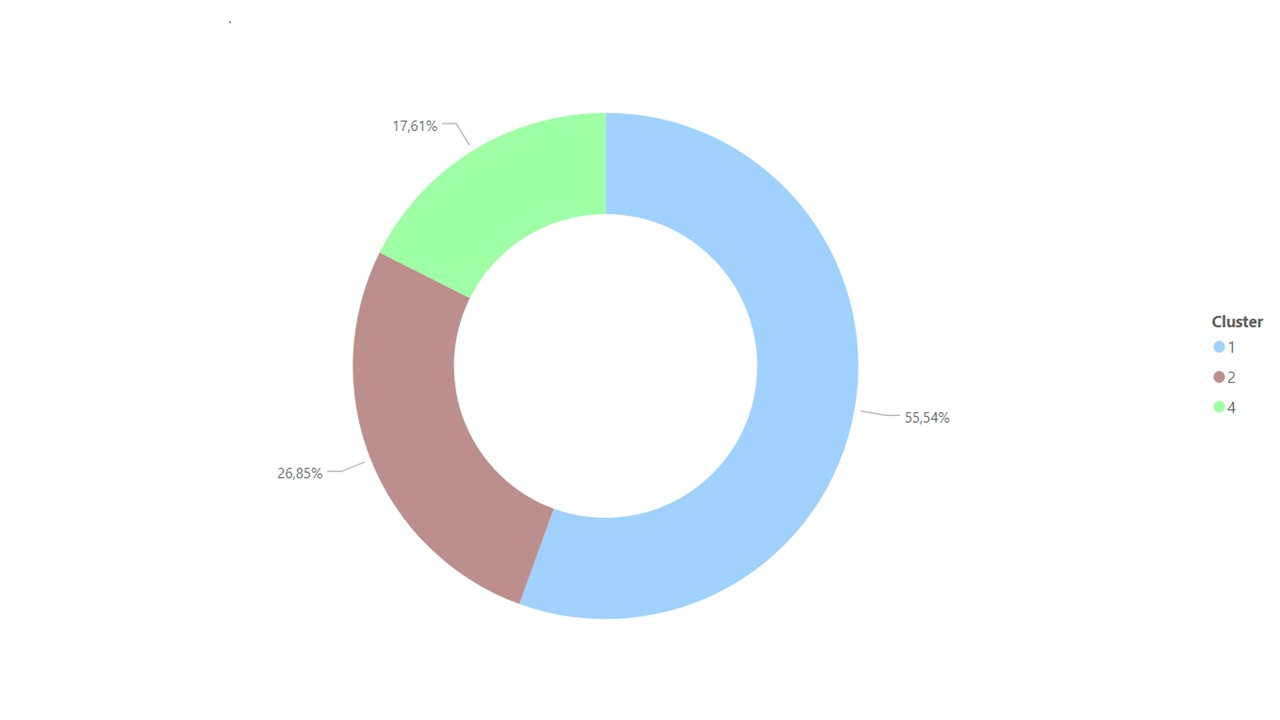
\includegraphics[width=\linewidth]{agglomerative_diagram_1}
\caption{Total net for each cluster.}
\label{fig:agglomerative2}
\end{subfigure}%
\caption{Descriptive statistics of the clusters.}
\label{fig:agglomerative_descriptives}
\end{figure}
\\
The importance of cluster 'Luxury vacation' on the total net is even more prominent now, as can be noticed from diagram \ref{agglomerative_diagram_1}. On the other side, the 'Low cost trip' cluster, even though it contains the most reservations, has a very low impact on the total revenue of the agency. Therefore, as proposed in the previous section the agency should concetrate more on the providance of the services of the clusters 'Luxury trip' and 'Relaxing vacation' and their promotion.